\documentclass[11pt]{article}
\pagestyle{empty}
\usepackage{graphicx}
\usepackage{amsmath}
\usepackage{tikz}
\usepackage{listings}% For displaying R code
\usepackage{mdframed}% For boxes
\textheight = 50 \baselineskip \textwidth 470pt \hoffset = -.8in
\voffset = -1in
\newcommand{\nin}{\noindent}


\begin{document}
\noindent {\bf MATH 140 \hskip.5in Name \underbar{\hskip2in} \hskip1in Date:}

\noindent{\bf Worksheet: US Governors 2021}

\medskip

\hrule
\vskip.5em
\nin {\bf The Scene}: We investigate a data set giving information about the current Governors of the 50 US States.
\medskip 
\nin {\bf The data matrix} appears on the last page of this worksheet.

\hrule
\medskip

\begin{enumerate}

\item How many observations does this data set have?  How many variables?  Classify each variable as numerical or categorical.

\vskip4em


\item Below is a bar chart generated in RStudio in an effort to investigate whether there is an association between the \texttt{party} and \texttt{region} categorical variables of this data set.
  
\parbox{3in}{
\begin{enumerate}
\item How many states are in the Mid-West region (MW)?  What proportion of these states has a Republican governor?

\vskip3em
\item What proportion of governors in the south east (SE) are Republican?

\vskip3em

\item If you pick a governor at random from the Mid-Atlantic region (MAtl), how likely is it that the governor would be Republican?
\vskip3em

\end{enumerate}}
\parbox{3.5in}{
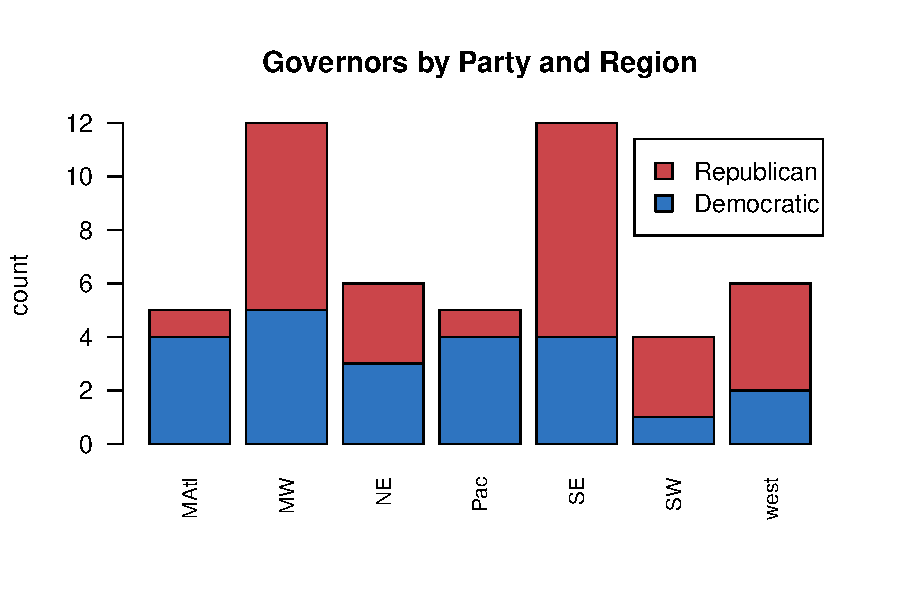
\includegraphics[width=3.5in]{stack_bar_party_region}}


\item Use the contingency table below to answer the following questions.

\begin{table}[ht]
	\centering
	\begin{tabular}{rrr} \hline
 	& F & M \\ \hline
	Democratic &   6 &  17 \\ 
  	Republican &   3 &  24 \\ \hline
	\end{tabular}
\end{table}

\begin{enumerate}
\item What proportion of governors are female?
\vskip3em
\item What proportion of governors are republican?
\vskip3em
\item What proportion of female governors are republican?
\vskip3em
\item What proportion of republican governors are male?
\vskip3em
\end{enumerate}



\item The \texttt{miss$\_$riv} variable is categorical, with possible values `W' or `E', depending on whether the state is west or east of the Mississippi River.  You will notice this column has been left blank, mostly.  Fill it in!  In the end, you should have 26 `E's and 24 `W's.


\item Determine 5 number summaries for the ages of governors west of the Mississippi, and 5 number summaries for the ages of governors east of the Mississippi.


\vskip10em

\item Draw side by side boxplots to make it visually easy to compare these two distributions.


\vskip10em

\item Does one region \textit{tend} to have older governors than the other? Explain.



\vskip5em

\item If you picked a state from the West at random, and a state from the East at random, which state would you expect to have an older governor?  Explain.


\vskip5em


\item We can also group the data according to their political party.  Here are side-by-side boxplots of governor ages grouped by party.  If you picked a governor at random from each political party, which governor would you expect to be older?  How confident would you be of your choice?


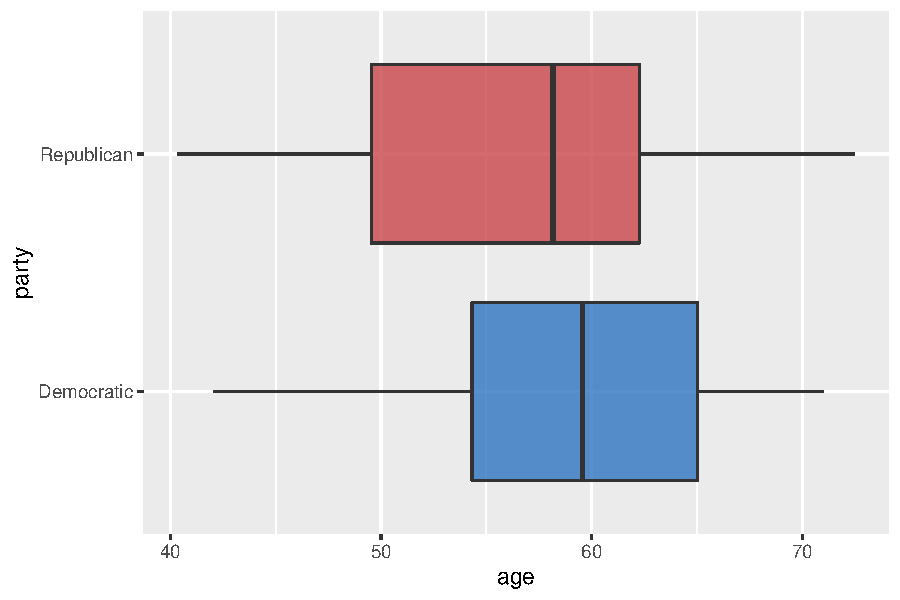
\includegraphics[width=3in]{box_age_by_party}

 \end{enumerate}

\vskip5em


%\begin{mdframed}{Sample code in R for inputing the dataset, and generating the plots in this worksheet]}
%\small{
%\begin{lstlisting}[language=R]

%#load the graphics package ggplot2, which we use for the box plot.
%library(ggplot2) 

%#input the csv file from my working directory and call it "gov"
%gov <- read.csv("governors.csv") 

%# fancy colors for democratic and republican parties
%party_colors <- c("#2E74C0", "#CB454A") 

%#stacked bar plot of governor party affiliation within regions
%barplot(table(gov$party, gov$region),
%       col=party_colors,
%        ylab="count",
 %       main="Governors by Party and Region",
%        legend=TRUE,
%        las=2,
%        cex.names = .8)
        
%# Box plots of age of governor by party
%ggplot(gov, aes(x=party, y=age)) + 
%  geom_boxplot(fill=party_colors, alpha=.8) +
%  coord_flip()
%\end{lstlisting}}
%\end{mdframed}



\newpage

\begin{table}[ht]
\centering
\begin{tabular}{rll c   | c |  ccl}
  \hline
 & state & governor & age.at.inaug & miss\_riv & region & sex & party \\ 
  \hline
1 & Alabama & Kay Ivey & 72 & ~E~ & SE & F & Republican \\ 
  2 & Alaska & Mike Dunleavy & 58 & W & Pac & M & Republican \\ 
  3 & Arizona & Doug Ducey & 51 &  & SW & M & Republican \\ 
  4 & Arkansas & Asa Hutchinson & 64 &  & SE & M & Republican \\ 
  5 & California & Gavin Newsom & 51 &  & Pac & M & Democratic \\ 
  6 & Colorado & Jared Polis & 44 &  & west & M & Democratic \\ 
  7 & Connecticut & Ned Lamont & 65 &  & NE & M & Democratic \\ 
  8 & Delaware & John Carney & 61 &  & MAtl & M & Democratic \\ 
  9 & Florida & Ron DeSantis & 40 &  & SE & M & Republican \\ 
  10 & Georgia & Brian Kemp & 55 &  & SE & M & Republican \\ 
  11 & Hawaii & David Ige & 58 &  & Pac & M & Democratic \\ 
  12 & Idaho & Brad Little & 65 &  & west & M & Republican \\ 
  13 & Illinois & J. B. Pritzker & 54 &  & MW & M & Democratic \\ 
  14 & Indiana & Eric Holcomb & 49 &  & MW & M & Republican \\ 
  15 & Iowa & Kim Reynolds & 58 &  & MW & F & Republican \\ 
  16 & Kansas & Laura Kelly & 69 &  & MW & F & Democratic \\ 
  17 & Kentucky & Andy Beshear & 42 &  & SE & M & Democratic \\ 
  18 & Louisiana & John Bel Edwards & 49 &  & SE & M & Democratic \\ 
  19 & Maine & Janet Mills & 71 &  & NE & F & Democratic \\ 
  20 & Maryland & Larry Hogan & 59 &  & MAtl & M & Republican \\ 
  21 & Massachusetts & Charlie Baker & 58 &  & NE & M & Republican \\ 
  22 & Michigan & Gretchen Whitmer & 47 &  & MW & F & Democratic \\ 
  23 & Minnesota & Tim Walz & 55 &  & MW & M & Democratic \\ 
  24 & Mississippi & Tate Reeves & 46 &  & SE & M & Republican \\ 
  25 & Missouri & Mike Parson & 63 &  & MW & M & Republican \\ 
  26 & Montana & Greg Gianforte & 60 &  & west & M & Republican \\ 
  27 & Nebraska & Pete Ricketts & 50 &  & MW & M & Republican \\ 
  28 & Nevada & Steve Sisolak & 65 &  & west & M & Democratic \\ 
  29 & New Hampshire & Chris Sununu & 42 &  & NE & M & Republican \\ 
  30 & New Jersey & Phil Murphy & 60 &  & MAtl & M & Democratic \\ 
  31 & New Mexico & Michelle L. Grisham & 59 &  & SW & F & Democratic \\ 
  32 & New York & Kathy Hochul & 63 &  & MAtl & F & Democratic \\ 
  33 & North Carolina & Roy Cooper & 60 &  & SE & M & Democratic \\ 
  34 & North Dakota & Doug Burgum & 60 &  & MW & M & Republican \\ 
  35 & Ohio & Mike DeWine & 72 &  & MW & M & Republican \\ 
  36 & Oklahoma & Kevin Stitt & 46 &  & SW & M & Republican \\ 
  37 & Oregon & Kate Brown & 55 &  & Pac & F & Democratic \\ 
  38 & Pennsylvania & Tom Wolf & 66 &  & MAtl & M & Democratic \\ 
  39 & Rhode Island & Daniel McKee & 70 &  & NE & M & Democratic \\ 
  40 & South Carolina & Henry McMaster & 70 &  & SE & M & Republican \\ 
  41 & South Dakota & Kristi Noem & 47 &  & MW & F & Republican \\ 
  42 & Tennessee & Bill Lee & 59 &  & SE & M & Republican \\ 
  43 & Texas & Greg Abbott & 57 &  & SW & M & Republican \\ 
  44 & Utah & Spencer Cox & 45 &  & west & M & Republican \\ 
  45 & Vermont & Phil Scott & 58 &  & NE & M & Republican \\ 
  46 & Virginia & Ralph Northam & 58 &  & SE & M & Democratic \\ 
  47 & Washington & Jay Inslee & 62 &  & Pac & M & Democratic \\ 
  48 & West Virginia & Jim Justice & 66 &  & SE & M & Republican \\ 
  49 & Wisconsin & Tony Evers & 67 &  & MW & M & Democratic \\ 
  50 & Wyoming & Mark Gordon & 62 &  & west & M & Republican \\ 
   \hline
\end{tabular}
\end{table}


\newpage

\begin{table}[ht]
\centering
\begin{tabular}{rll c cccl}
  \hline
 & state & governor & age.at.inaug & miss\_riv & region & sex & party \\ 
  \hline
1 & Alabama & Kay Ivey & 72 & E & SE & F & Republican \\ 
  2 & Alaska & Mike Dunleavy & 58 & W & Pac & M & Republican \\ 
  3 & Arizona & Doug Ducey & 51 & W & SW & M & Republican \\ 
  4 & Arkansas & Asa Hutchinson & 64 & W & SE & M & Republican \\ 
  5 & California & Gavin Newsom & 51 & W & Pac & M & Democratic \\ 
  6 & Colorado & Jared Polis & 44 & W & west & M & Democratic \\ 
  7 & Connecticut & Ned Lamont & 65 & E & NE & M & Democratic \\ 
  8 & Delaware & John Carney & 61 & E & MAtl & M & Democratic \\ 
  9 & Florida & Ron DeSantis & 40 & E & SE & M & Republican \\ 
  10 & Georgia & Brian Kemp & 55 & E & SE & M & Republican \\ 
  11 & Hawaii & David Ige & 58 & W & Pac & M & Democratic \\ 
  12 & Idaho & Brad Little & 65 & W & west & M & Republican \\ 
  13 & Illinois & J. B. Pritzker & 54 & E & MW & M & Democratic \\ 
  14 & Indiana & Eric Holcomb & 49 & E & MW & M & Republican \\ 
  15 & Iowa & Kim Reynolds & 58 & W & MW & F & Republican \\ 
  16 & Kansas & Laura Kelly & 69 & W & MW & F & Democratic \\ 
  17 & Kentucky & Andy Beshear & 42 & E & SE & M & Democratic \\ 
  18 & Louisiana & John Bel Edwards & 49 & W & SE & M & Democratic \\ 
  19 & Maine & Janet Mills & 71 & E & NE & F & Democratic \\ 
  20 & Maryland & Larry Hogan & 59 & E & MAtl & M & Republican \\ 
  21 & Massachusetts & Charlie Baker & 58 & E & NE & M & Republican \\ 
  22 & Michigan & Gretchen Whitmer & 47 & E & MW & F & Democratic \\ 
  23 & Minnesota & Tim Walz & 55 & W & MW & M & Democratic \\ 
  24 & Mississippi & Tate Reeves & 46 & E & SE & M & Republican \\ 
  25 & Missouri & Mike Parson & 63 & W & MW & M & Republican \\ 
  26 & Montana & Greg Gianforte & 60 & W & west & M & Republican \\ 
  27 & Nebraska & Pete Ricketts & 50 & W & MW & M & Republican \\ 
  28 & Nevada & Steve Sisolak & 65 & W & west & M & Democratic \\ 
  29 & New Hampshire & Chris Sununu & 42 & E & NE & M & Republican \\ 
  30 & New Jersey & Phil Murphy & 60 & E & MAtl & M & Democratic \\ 
  31 & New Mexico & Michelle L. Grisham & 59 & W & SW & F & Democratic \\ 
  32 & New York & Kathy Hochul & 63 & E & MAtl & F & Democratic \\ 
  33 & North Carolina & Roy Cooper & 60 & E & SE & M & Democratic \\ 
  34 & North Dakota & Doug Burgum & 60 & W & MW & M & Republican \\ 
  35 & Ohio & Mike DeWine & 72 & E & MW & M & Republican \\ 
  36 & Oklahoma & Kevin Stitt & 46 & W & SW & M & Republican \\ 
  37 & Oregon & Kate Brown & 55 & W & Pac & F & Democratic \\ 
  38 & Pennsylvania & Tom Wolf & 66 & E & MAtl & M & Democratic \\ 
  39 & Rhode Island & Daniel McKee & 70 & E & NE & M & Democratic \\ 
  40 & South Carolina & Henry McMaster & 70 & E & SE & M & Republican \\ 
  41 & South Dakota & Kristi Noem & 47 & W & MW & F & Republican \\ 
  42 & Tennessee & Bill Lee & 59 & E & SE & M & Republican \\ 
  43 & Texas & Greg Abbott & 57 & W & SW & M & Republican \\ 
  44 & Utah & Spencer Cox & 45 & W & west & M & Republican \\ 
  45 & Vermont & Phil Scott & 58 & E & NE & M & Republican \\ 
  46 & Virginia & Ralph Northam & 58 & E & SE & M & Democratic \\ 
  47 & Washington & Jay Inslee & 62 & W & Pac & M & Democratic \\ 
  48 & West Virginia & Jim Justice & 66 & E & SE & M & Republican \\ 
  49 & Wisconsin & Tony Evers & 67 & E & MW & M & Democratic \\ 
  50 & Wyoming & Mark Gordon & 62 & W & west & M & Republican \\ 
   \hline
\end{tabular}
\end{table}




\end{document}
